% =============================================================================
% Paper 4: QCanvas IDE -- A Web-Based Quantum Computing Development
%          Environment for Education and Research
% =============================================================================
\documentclass[conference]{IEEEtran}

% --- Packages ----------------------------------------------------------------
\usepackage{cite}
\usepackage{amsmath,amssymb,amsfonts}
\usepackage{graphicx}
\usepackage{textcomp}
\usepackage{xcolor}
\usepackage{listings}
\usepackage{booktabs}
\usepackage{multirow}
\usepackage{hyperref}
\usepackage{tikz}
\usepackage{subcaption}
\usepackage{balance}
\usepackage{enumitem}
\usepackage{tabularx}

\usetikzlibrary{shapes, arrows.meta, positioning, fit, backgrounds}

% --- Listings Configuration --------------------------------------------------
\lstset{
  basicstyle=\ttfamily\footnotesize,
  keywordstyle=\color{blue}\bfseries,
  commentstyle=\color{gray}\itshape,
  stringstyle=\color{red},
  numbers=left,
  numberstyle=\tiny\color{gray},
  stepnumber=1,
  numbersep=5pt,
  frame=single,
  breaklines=true,
  captionpos=b,
  tabsize=2,
  showstringspaces=false,
}

% --- Title -------------------------------------------------------------------
\title{QCanvas IDE: A Web-Based Quantum Computing\\Development Environment for Education and Research}

\author{
  \IEEEauthorblockN{Umer Farooq\IEEEauthorrefmark{1},
  Hussan Waseem Syed\IEEEauthorrefmark{1},
  Muhammad Irtaza Khan\IEEEauthorrefmark{1}}
  \IEEEauthorblockA{\IEEEauthorrefmark{1}Department of Computer Science,
  FAST National University of Computer and Emerging Sciences, Islamabad, Pakistan\\
  \{i220891, i220893, i220911\}@nu.edu.pk}
  \and
  \IEEEauthorblockN{Dr.\ Imran Ashraf\IEEEauthorrefmark{2},
  Dr.\ Muhammad Nouman Noor\IEEEauthorrefmark{2}}
  \IEEEauthorblockA{\IEEEauthorrefmark{2}Faculty of Computing,
  FAST National University of Computer and Emerging Sciences, Islamabad, Pakistan}
}

\begin{document}
\maketitle

% =============================================================================
% ABSTRACT
% =============================================================================
\begin{abstract}
Quantum computing education faces a critical accessibility challenge: learners must navigate fragmented toolchains, complex local installations, and framework-specific syntaxes before they can explore fundamental quantum concepts. We present QCanvas~IDE, a web-based quantum computing development environment designed to serve both educational and research communities. QCanvas~IDE provides a unified browser-based workspace that supports three major quantum frameworks---Qiskit, Cirq, and PennyLane---with real-time compilation to OpenQASM~3.0, multi-backend quantum simulation, and interactive results visualization. The platform features an advanced Monaco-based code editor with syntax highlighting, a comprehensive keyboard shortcuts system, persistent user authentication, a curated library of 25+ pre-built quantum algorithm examples spanning six categories, and a multi-tab results panel with histogram visualization, execution statistics, and detailed error diagnostics. By lowering the barrier to entry through zero-installation access and progressive disclosure of complexity, QCanvas~IDE enables students, educators, and researchers to focus on quantum computing concepts rather than tooling. We describe the platform's design principles, architecture, feature set, and educational scaffolding strategies, and present preliminary evaluation through functional testing across 105 quantum circuits. QCanvas~IDE is developed under the Open Quantum Workbench initiative at FAST University and is available as open-source software.
\end{abstract}

\begin{IEEEkeywords}
quantum computing education, web-based IDE, OpenQASM 3.0, quantum simulation, interactive learning, Qiskit, Cirq, PennyLane
\end{IEEEkeywords}

% =============================================================================
% I. INTRODUCTION
% =============================================================================
\section{Introduction}
\label{sec:introduction}

Quantum computing is transitioning from a purely theoretical discipline to an applied technology with growing demand for skilled practitioners. University curricula increasingly include quantum computing courses~\cite{asfaw2022building}, and industry demand for quantum software developers continues to rise~\cite{fox2020preparing}. However, several barriers impede effective quantum computing education:

\begin{enumerate}[label=(\alph*)]
    \item \textbf{Installation complexity:} Setting up quantum SDKs (Qiskit, Cirq, PennyLane) with their numerous dependencies is time-consuming and error-prone, particularly for beginners.
    \item \textbf{Framework fragmentation:} Each framework uses different APIs, naming conventions, and paradigms, requiring learners to master framework-specific details before engaging with quantum concepts.
    \item \textbf{Lack of immediate feedback:} Command-line workflows provide poor interactive experiences; results require manual visualization.
    \item \textbf{No unified standard:} Students cannot easily compare how the same quantum algorithm is expressed across frameworks, limiting conceptual understanding.
    \item \textbf{Limited scaffolding:} Existing tools provide either oversimplified drag-and-drop interfaces (lacking real programming) or full SDKs (overwhelming for beginners).
\end{enumerate}

To address these challenges, we present \textbf{QCanvas~IDE}, a web-based quantum computing development environment that provides a unified, zero-installation workspace supporting all three major quantum frameworks with real-time compilation, simulation, and visualization. QCanvas~IDE is designed around three core principles:

\begin{itemize}
    \item \textbf{Progressive disclosure:} Hide complexity behind sensible defaults while making advanced features accessible.
    \item \textbf{Immediate feedback:} Provide real-time validation, compilation, and simulation results.
    \item \textbf{Multi-framework literacy:} Enable learners to see and compare quantum algorithms across frameworks and their standardized OpenQASM~3.0 representation.
\end{itemize}

The contributions of this paper are:
\begin{enumerate}
    \item The design and implementation of a web-based quantum IDE supporting three frameworks with real-time OpenQASM~3.0 compilation and multi-backend simulation.
    \item A curated example library of 25+ quantum algorithm implementations across six educational categories, designed for progressive learning.
    \item An analysis of educational design principles applied to quantum computing tooling, including progressive disclosure, scaffolded learning, and multi-framework comparison.
    \item A comprehensive feature set including authentication, file management, keyboard shortcuts, and customizable preferences tailored for both classroom and research use.
\end{enumerate}

% =============================================================================
% II. RELATED WORK
% =============================================================================
\section{Related Work}
\label{sec:related}

\subsection{Quantum Computing Educational Tools}

Several web-based tools exist for quantum computing education, each with different design philosophies:

\textbf{IBM Quantum Composer}~\cite{ibmquantum} provides a drag-and-drop circuit builder with access to real quantum hardware. While excellent for visual circuit construction, it is limited to the Qiskit ecosystem and does not support code-based workflows from other frameworks.

\textbf{Quirk}~\cite{quirk2016} is an open-source browser-based circuit simulator offering real-time state visualization. It uses a visual drag-and-drop interface but lacks support for code-based circuit definition, making it unsuitable for teaching programming-oriented quantum computing.

\textbf{Quantum Programming Studio}~\cite{davila2022quantum} provides a web IDE for quantum programming but supports only limited frameworks and lacks OpenQASM~3.0 compliance.

\textbf{Google Colab with Cirq} and \textbf{IBM Quantum Lab} (Jupyter-based) offer cloud-hosted notebook environments but are framework-specific, require authentication setup, and lack integrated results visualization.

\subsection{Comparison with QCanvas IDE}

Table~\ref{tab:toolcomparison} summarizes the comparison between QCanvas~IDE and existing tools:

\begin{table*}[t]
\centering
\caption{Comparison of Quantum Computing Educational Tools}
\label{tab:toolcomparison}
\begin{tabular}{@{}lccccccc@{}}
\toprule
\textbf{Feature} & \textbf{QCanvas} & \textbf{IBM Composer} & \textbf{Quirk} & \textbf{QP Studio} & \textbf{Colab+Cirq} & \textbf{IBM Q Lab} \\
\midrule
Web-based (zero install) & \checkmark & \checkmark & \checkmark & \checkmark & \checkmark & \checkmark \\
Multi-framework support  & \checkmark & --- & --- & Partial & --- & --- \\
Code-based editing       & \checkmark & Partial & --- & \checkmark & \checkmark & \checkmark \\
OpenQASM 3.0 output      & \checkmark & --- & --- & --- & --- & --- \\
Real-time simulation     & \checkmark & \checkmark & \checkmark & \checkmark & --- & \checkmark \\
Histogram visualization  & \checkmark & \checkmark & --- & Partial & Manual & \checkmark \\
Pre-built examples       & 25+ & \checkmark & --- & Limited & --- & \checkmark \\
Multi-backend simulation & \checkmark & --- & --- & --- & --- & --- \\
Keyboard shortcuts       & \checkmark & Partial & --- & --- & \checkmark & \checkmark \\
File management          & \checkmark & --- & --- & --- & \checkmark & \checkmark \\
Authentication system    & \checkmark & \checkmark & --- & --- & \checkmark & \checkmark \\
Educational scaffolding  & \checkmark & \checkmark & \checkmark & --- & --- & Partial \\
\bottomrule
\end{tabular}
\end{table*}

QCanvas~IDE uniquely combines multi-framework code editing, real-time OpenQASM~3.0 compilation, multi-backend simulation, and educational scaffolding in a single platform.

% =============================================================================
% III. DESIGN PRINCIPLES
% =============================================================================
\section{Educational Design Principles}
\label{sec:design}

QCanvas~IDE's design is grounded in established principles from computing education research:

\subsection{Progressive Disclosure}

Inspired by Shneiderman's information-seeking mantra~\cite{shneiderman1996eyes} (overview first, zoom and filter, details on demand), QCanvas~IDE presents a clean initial interface and progressively reveals complexity:

\begin{itemize}
    \item \textbf{Level 1 (Beginner):} Open a pre-built example, click ``Compile,'' view the QASM output and histogram. No configuration required.
    \item \textbf{Level 2 (Intermediate):} Edit code, select different frameworks, configure simulation shots, and compare results across backends.
    \item \textbf{Level 3 (Advanced):} Use keyboard shortcuts for rapid development, create multi-file projects, analyze execution statistics (gate counts, circuit depth, memory usage, fidelity), and examine detailed error diagnostics.
\end{itemize}

\subsection{Scaffolded Learning with Examples}

The example system is designed as an educational progression pathway:

\begin{table}[t]
\centering
\caption{Example Library Structure (25+ Examples)}
\label{tab:examples}
\begin{tabular}{@{}p{2.5cm}p{2.2cm}p{2.5cm}@{}}
\toprule
\textbf{Category} & \textbf{Difficulty} & \textbf{Examples} \\
\midrule
Basic Circuits       & Beginner     & Bell State, GHZ State \\
Quantum Algorithms   & Intermediate & Teleportation, Deutsch-Jozsa, QRNG, Grover's \\
Variational Alg.     & Advanced     & VQE, QAOA \\
Quantum ML           & Advanced     & QNN, XOR Classifier \\
Error Correction     & Advanced     & Bit-flip code \\
Cross-Framework      & All levels   & Same algorithm in Qiskit, Cirq, PennyLane \\
\bottomrule
\end{tabular}
\end{table}

Each example category builds upon concepts from previous categories. Critically, several algorithms (Teleportation, Deutsch-Jozsa, QRNG, Grover's) are provided in \emph{all three frameworks}, enabling direct comparison of how different SDKs express the same quantum computation.

\subsection{Immediate Feedback Loops}

Following Constructionist learning theory~\cite{papert1991situating}, where learners construct knowledge through building and testing artifacts, QCanvas~IDE provides immediate feedback at every step:

\begin{itemize}
    \item \textbf{Syntax validation:} Real-time error highlighting during code editing.
    \item \textbf{Compilation feedback:} Step-by-step console logging showing parsing, analysis, and generation stages.
    \item \textbf{Simulation results:} Measurement histograms rendered within seconds.
    \item \textbf{Error diagnostics:} Detailed error messages with code snippets and fix suggestions.
    \item \textbf{Statistics:} Gate counts, circuit depth, qubit utilization, execution time, and memory usage displayed alongside results.
\end{itemize}

\subsection{Multi-Framework Literacy}

Rather than locking students into a single framework, QCanvas~IDE promotes \emph{multi-framework literacy}:

\begin{itemize}
    \item Students see that a Hadamard gate is \texttt{qc.h(0)} in Qiskit, \texttt{cirq.H(q0)} in Cirq, and \texttt{qml.Hadamard(wires=0)} in PennyLane---but they all compile to \texttt{h q[0];} in OpenQASM~3.0.
    \item This reinforces that quantum concepts are \emph{framework-independent}, building deeper conceptual understanding.
    \item The OpenQASM~3.0 intermediate representation serves as a ``Rosetta Stone'' for quantum programming.
\end{itemize}

% =============================================================================
% IV. SYSTEM ARCHITECTURE
% =============================================================================
\section{System Architecture}
\label{sec:architecture}

QCanvas~IDE employs a hybrid architecture (Figure~\ref{fig:architecture}) with clear separation between frontend presentation, backend computation, and quantum processing:

\begin{figure}[t]
\centering
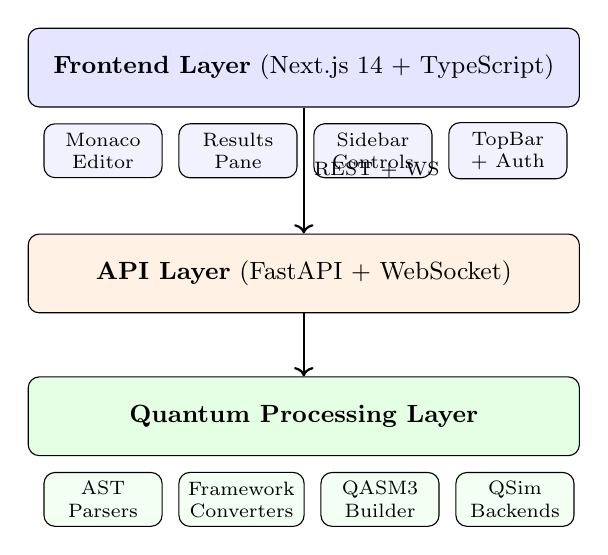
\begin{tikzpicture}[
    node distance=0.8cm,
    layer/.style={rectangle, draw, rounded corners, minimum width=7cm, minimum height=1.0cm, align=center, font=\small},
    component/.style={rectangle, draw, rounded corners, minimum width=1.5cm, minimum height=0.6cm, align=center, font=\scriptsize},
    arrow/.style={->, thick}
]

% Frontend layer
\node[layer, fill=blue!10] (frontend) {\textbf{Frontend Layer} (Next.js 14 + TypeScript)};
\node[component, below=0.2cm of frontend.south west, anchor=north west, xshift=0.2cm, fill=blue!5] (editor) {Monaco\\Editor};
\node[component, right=0.2cm of editor, fill=blue!5] (results) {Results\\Pane};
\node[component, right=0.2cm of results, fill=blue!5] (sidebar) {Sidebar\\Controls};
\node[component, right=0.2cm of sidebar, fill=blue!5] (topbar) {TopBar\\+ Auth};

% API layer
\node[layer, fill=orange!10, below=1.6cm of frontend] (api) {\textbf{API Layer} (FastAPI + WebSocket)};

% Processing layer
\node[layer, fill=green!10, below=0.8cm of api] (processing) {\textbf{Quantum Processing Layer}};
\node[component, below=0.2cm of processing.south west, anchor=north west, xshift=0.2cm, fill=green!5] (parsers) {AST\\Parsers};
\node[component, right=0.2cm of parsers, fill=green!5] (converters) {Framework\\Converters};
\node[component, right=0.2cm of converters, fill=green!5] (qasm) {QASM3\\Builder};
\node[component, right=0.2cm of qasm, fill=green!5] (qsim) {QSim\\Backends};

% Arrows
\draw[arrow] (frontend) -- node[right, font=\scriptsize] {REST + WS} (api);
\draw[arrow] (api) -- (processing);

\end{tikzpicture}
\caption{QCanvas IDE three-layer architecture.}
\label{fig:architecture}
\end{figure}

\subsection{Frontend (Next.js 14)}

The frontend is built with Next.js~14 using the App Router, React~18, TypeScript, and Tailwind~CSS. Key components include:

\subsubsection{Monaco Editor Integration}
The code editor uses Microsoft's Monaco Editor (the engine behind VS Code), providing:
\begin{itemize}
    \item Syntax highlighting for Python, with framework-specific keyword recognition.
    \item Multi-file workspace with tabbed navigation.
    \item Find and replace functionality.
    \item Automatic file type detection.
\end{itemize}

\subsubsection{Multi-Tab Results Panel}
The results pane provides five specialized tabs:
\begin{itemize}
    \item \textbf{Stats:} Gradient-colored hero cards showing gate counts, circuit depth, qubit count, and performance metrics (execution time, memory, CPU usage, fidelity).
    \item \textbf{Console:} Step-by-step execution log showing parsing, analysis, and generation stages with timing information.
    \item \textbf{Errors:} Detailed error display with source code snippets, line numbers, and fix suggestions.
    \item \textbf{Histogram:} Chart.js-powered histogram visualization of measurement outcomes with percentage labels and progress bars.
    \item \textbf{Output:} Raw OpenQASM~3.0 output and simulation results.
\end{itemize}

\subsubsection{Simulation Controls}
An integrated control panel allows configuration of:
\begin{itemize}
    \item Input framework selection (Qiskit, Cirq, PennyLane, QASM).
    \item Simulation backend selection (Cirq, Qiskit, PennyLane backends via QSim).
    \item Shot count configuration (1--10,000).
    \item Execution mode: Compile Only, Execute, or Hybrid execution.
\end{itemize}

\subsection{Backend (FastAPI)}

The backend provides:
\begin{itemize}
    \item RESTful API endpoints for compilation (\texttt{/api/converter/convert}) and simulation (\texttt{/api/simulator/execute}).
    \item WebSocket endpoint (\texttt{/ws}) for real-time progress updates during long-running operations.
    \item Pydantic-based request/response validation.
    \item Automatic OpenAPI documentation at \texttt{/docs}.
\end{itemize}

\subsection{Quantum Processing Layer}

The processing layer implements:
\begin{itemize}
    \item AST-based parsers for Qiskit, Cirq, and PennyLane (secure, no code execution).
    \item A unified Circuit~AST intermediate representation.
    \item QASM3Builder infrastructure for OpenQASM~3.0 code generation.
    \item QSim integration for multi-backend simulation.
\end{itemize}

% =============================================================================
% V. KEY FEATURES
% =============================================================================
\section{Platform Features}
\label{sec:features}

\subsection{Authentication and User Management}

QCanvas~IDE implements a persistent authentication system to support classroom deployment:

\begin{itemize}
    \item \textbf{User registration and login} with session persistence via localStorage.
    \item \textbf{Demo account} (\texttt{demo@qcanvas.dev}) for instant access without registration.
    \item \textbf{Conditional UI rendering:} Login/logout buttons, user profile display, and feature gating based on authentication status.
    \item \textbf{Automatic redirect} for authenticated users from the login page to the workspace.
    \item \textbf{Role-based access control} for future classroom features (instructor/student roles).
\end{itemize}

\subsection{Comprehensive Keyboard Shortcuts}

To support efficient workflows for power users and researchers, QCanvas~IDE provides 10+ keyboard shortcuts:

\begin{table}[t]
\centering
\caption{QCanvas IDE Keyboard Shortcuts}
\label{tab:shortcuts}
\begin{tabular}{@{}ll@{}}
\toprule
\textbf{Shortcut} & \textbf{Action} \\
\midrule
Ctrl/Cmd + S           & Save current file \\
Ctrl/Cmd + N           & Create new file (auto-named) \\
Ctrl/Cmd + B           & Toggle sidebar visibility \\
Ctrl/Cmd + J           & Toggle results panel \\
Ctrl/Cmd + F           & Find in code \\
Ctrl/Cmd + H           & Find and replace \\
Ctrl/Cmd + Shift + K   & Toggle dark/light theme \\
Ctrl/Cmd + Shift + R   & Compile and run circuit \\
Ctrl/Cmd + Tab         & Switch to next file tab \\
Ctrl/Cmd + Shift + Tab & Switch to previous file tab \\
\bottomrule
\end{tabular}
\end{table}

The shortcut system uses React \texttt{useEffect}-based event listeners with proper cleanup, cross-platform support (detecting Ctrl vs.\ Cmd), and prevention of default browser behaviors.

\subsection{Example System with Smart Loading}

The example system is a key educational feature designed for discoverability and seamless integration:

\begin{enumerate}
    \item \textbf{Homepage example cards:} Visual cards displaying algorithm name, framework, difficulty level, and a brief description. Clicking a card initiates the smart loading flow.
    \item \textbf{Authentication-aware loading:} If the user is authenticated, the example code is injected directly into the editor workspace. If not, the code is stored in session storage, and the user is redirected to login first.
    \item \textbf{Automatic code injection:} After authentication, session-stored example code is automatically loaded into a new editor tab with appropriate framework detection.
    \item \textbf{Framework diversity:} Examples are distributed across all three frameworks to encourage exploration.
\end{enumerate}

\subsection{File Management and Templates}

The file management system supports multi-file quantum projects:

\begin{itemize}
    \item \textbf{Initial files:} Three files auto-loaded on first use---Bell State (Cirq), Deutsch-Jozsa (Qiskit), Grover's Search (PennyLane)---providing immediate hands-on content.
    \item \textbf{File templates:} Additional templates available via modal---Teleportation (Qiskit), QRNG (Cirq), XOR Demo (PennyLane), QML XOR Classifier (PennyLane).
    \item \textbf{Automatic naming:} New files receive sequential names (\texttt{circuit\_1.py}, \texttt{circuit\_2.py}).
    \item \textbf{Custom delete confirmation:} Themed modal dialogs replace browser \texttt{confirm()} for consistent UX.
    \item \textbf{Click-outside-to-close:} All modals dismiss when clicking the backdrop.
\end{itemize}

\subsection{Settings and Preferences}

Persistent user preferences include:
\begin{itemize}
    \item \textbf{Theme selection:} Dark and light modes with smooth transitions.
    \item \textbf{Auto-save:} Toggleable automatic file saving.
    \item \textbf{Format on save:} Automatic code formatting.
    \item Settings persist across sessions via localStorage.
\end{itemize}

\subsection{Results Visualization and Analysis}

The results panel provides rich feedback for educational and research use:

\subsubsection{Statistics Panel}
Gradient-colored cards display:
\begin{itemize}
    \item Circuit metrics: gate count, circuit depth, qubit count.
    \item Performance metrics: execution time (ms), memory usage (MB), CPU utilization (\%).
    \item Quantum metrics: estimated fidelity.
    \item Color-coded indicators: green (good), yellow (moderate), red (needs attention).
\end{itemize}

\subsubsection{Histogram Visualization}
Measurement results are displayed as:
\begin{itemize}
    \item Bar chart with outcome labels (\texttt{00}, \texttt{01}, \texttt{10}, \texttt{11}).
    \item Percentage labels on each bar.
    \item Visual progress bars below the chart.
    \item Rendered using Chart.js for interactive exploration.
\end{itemize}

\subsubsection{Console Logging}
Step-by-step compilation logs show:
\begin{itemize}
    \item Framework detection and parser selection.
    \item AST parsing progress with timing.
    \item Circuit analysis results.
    \item QASM generation stages.
    \item Simulation execution progress.
\end{itemize}

\subsubsection{Error Diagnostics}
When errors occur, the Errors tab displays:
\begin{itemize}
    \item Error type and message.
    \item Source code snippet with the problematic line highlighted.
    \item Suggested fixes based on common error patterns.
    \item Framework-specific guidance.
\end{itemize}

% =============================================================================
% VI. HYBRID EXECUTION MODEL
% =============================================================================
\section{Hybrid Execution Model}
\label{sec:execution}

QCanvas~IDE supports three execution modes, enabling different educational scenarios:

\subsection{Compile Only Mode}
Converts framework code to OpenQASM~3.0 without simulation. Useful for:
\begin{itemize}
    \item Teaching OpenQASM~3.0 syntax by showing compilation output.
    \item Understanding how high-level gates decompose to standard gate sets.
    \item Comparing QASM output across frameworks for the same algorithm.
\end{itemize}

\subsection{Full Execute Mode}
Compiles to OpenQASM~3.0 and runs simulation via QSim backend. Supports:
\begin{itemize}
    \item Multiple backends (Cirq, Qiskit, PennyLane simulators).
    \item Configurable shot counts for statistical analysis.
    \item Measurement histogram visualization.
\end{itemize}

\subsection{Hybrid Execute Mode}
Executes Python code with access to \texttt{qcanvas.compile()} and \texttt{qsim.run()} APIs:

\begin{lstlisting}[language=Python, caption={Hybrid execution example}]
import cirq
from qcanvas import compile
import qsim

# Create circuit
q0, q1 = cirq.LineQubit.range(2)
circuit = cirq.Circuit(
    cirq.H(q0), cirq.CNOT(q0, q1),
    cirq.measure(q0, q1, key='result'))

# Compile to QASM
qasm = compile(circuit, framework="cirq")
print(f"Generated QASM:\n{qasm}")

# Execute simulations
for i in range(3):
    result = qsim.run(qasm, shots=100,
                      backend="cirq")
    print(f"Run {i+1}: {result.counts}")
\end{lstlisting}

This mode runs in a sandboxed environment with configurable security:
\begin{itemize}
    \item Blocked imports: \texttt{os}, \texttt{subprocess}, \texttt{sys}, \texttt{socket}.
    \item Prohibited: file access, network access, shell commands.
    \item Allowed: \texttt{cirq}, \texttt{qiskit}, \texttt{pennylane}, \texttt{numpy}, \texttt{math}, \texttt{qcanvas}, \texttt{qsim}.
    \item Timeout and memory limits enforced.
    \item Print statements captured and displayed in Output tab.
\end{itemize}

% =============================================================================
% VII. EDUCATIONAL USE CASES
% =============================================================================
\section{Educational Use Cases}
\label{sec:usecases}

\subsection{Introductory Quantum Computing Course}

\textbf{Scenario:} A university instructor teaches a first course in quantum computing.

\textbf{Workflow:}
\begin{enumerate}
    \item Students access QCanvas~IDE through any web browser---no installation required.
    \item Students log in with demo accounts or registered accounts.
    \item Instructor assigns the Bell State example (auto-loaded as initial file).
    \item Students click ``Compile'' to see OpenQASM~3.0 output, learning the standard gate language.
    \item Students click ``Execute'' to see the $|00\rangle$ and $|11\rangle$ measurement histogram, reinforcing entanglement concepts.
    \item Students modify the circuit (e.g., add a Z gate) and immediately see how results change.
\end{enumerate}

\subsection{Cross-Framework Comparison Lab}

\textbf{Scenario:} Students compare quantum teleportation across frameworks.

\textbf{Workflow:}
\begin{enumerate}
    \item From the Examples page, students load ``Quantum Teleportation (Qiskit).''
    \item They compile and examine the QASM output.
    \item They then load ``Quantum Teleportation (Cirq)'' and ``Quantum Teleportation (PennyLane)'' in separate file tabs.
    \item Side-by-side comparison reveals that despite different Python syntax, the underlying quantum operations (and QASM output) are equivalent.
    \item This reinforces that quantum computing concepts are framework-independent.
\end{enumerate}

\subsection{Research Algorithm Development}

\textbf{Scenario:} A researcher develops a variational quantum algorithm.

\textbf{Workflow:}
\begin{enumerate}
    \item Use the VQE or QAOA example as a starting template.
    \item Modify the ansatz and cost function.
    \item Use Hybrid Execute mode with loop-based multi-simulation to collect statistics.
    \item Analyze results through the histogram and statistics panels.
    \item Export QASM code for use in external tools or hardware submissions.
\end{enumerate}

\subsection{Quantum Machine Learning Workshop}

\textbf{Scenario:} A workshop on quantum machine learning using PennyLane.

\textbf{Workflow:}
\begin{enumerate}
    \item Participants load the ``QML XOR Classifier'' PennyLane example.
    \item They observe the quantum neural network architecture in the code.
    \item Using Hybrid Execute mode, they run the training loop and see classification results.
    \item They experiment with different ansatz structures and gate parameters.
    \item The QCanvas compile step shows how variational circuits map to standard gates.
\end{enumerate}

% =============================================================================
% VIII. EVALUATION
% =============================================================================
\section{Evaluation}
\label{sec:evaluation}

\subsection{Functional Testing}

QCanvas~IDE has been validated through a comprehensive test suite:

\begin{table}[t]
\centering
\caption{Test Suite Results}
\label{tab:tests}
\begin{tabular}{@{}lrr@{}}
\toprule
\textbf{Test Category} & \textbf{Count} & \textbf{Pass Rate} \\
\midrule
Iteration I unit tests       & 48 & 100\% \\
Cirq integration             & 7  & 100\% \\
Qiskit integration           & 8  & 100\% \\
PennyLane Iteration I        & 7  & 100\% \\
PennyLane Iteration II       & 8  & 100\% \\
Gate modifiers               & 7  & 100\% \\
Language features             & 15 & 100\% \\
Expected failures (xfail)    & 4  & N/A \\
Skipped (future features)    & 29 & N/A \\
\midrule
\textbf{Total (excl.\ skip/xfail)} & \textbf{100} & \textbf{100\%} \\
\bottomrule
\end{tabular}
\end{table}

\subsection{Performance Characteristics}

\begin{table}[t]
\centering
\caption{Platform Performance Metrics}
\label{tab:performance}
\begin{tabular}{@{}lr@{}}
\toprule
\textbf{Metric} & \textbf{Value} \\
\midrule
Average compilation time     & $<$50\,ms \\
Average simulation time (1024 shots) & $<$2\,s \\
Frontend initial load time   & $<$3\,s \\
API response time (simple)   & $<$200\,ms \\
WebSocket latency            & $<$100\,ms \\
\bottomrule
\end{tabular}
\end{table}

\subsection{Feature Coverage}

QCanvas~IDE supports:
\begin{itemize}
    \item \textbf{44/44} Iteration I OpenQASM~3.0 features (100\%).
    \item \textbf{All} Iteration II features: advanced modifiers, subroutines, complex types, bitwise operations, while/break/continue.
    \item \textbf{25+} pre-built examples across 6 categories and 3 frameworks.
    \item \textbf{3} simulation backends with configurable parameters.
\end{itemize}

\subsection{Limitations and Future User Study}

We acknowledge that a formal user study with students and educators has not yet been conducted. Such a study is planned as immediate future work and would evaluate:
\begin{itemize}
    \item Task completion time for common quantum programming exercises.
    \item System Usability Scale (SUS) scores.
    \item Learning outcomes compared to traditional SDK-based instruction.
    \item Cognitive load measurements (NASA-TLX).
    \item Qualitative feedback on educational scaffolding effectiveness.
\end{itemize}

% =============================================================================
% IX. DEPLOYMENT
% =============================================================================
\section{Deployment}
\label{sec:deployment}

QCanvas~IDE supports multiple deployment modes:

\begin{itemize}
    \item \textbf{Docker Compose:} Full-stack deployment with PostgreSQL, Redis, backend, frontend, Nginx reverse proxy, Prometheus, and Grafana monitoring.
    \item \textbf{Local development:} Separate backend (Uvicorn) and frontend (Next.js dev server) processes.
    \item \textbf{Linux quick setup:} Automated \texttt{setup.sh} and \texttt{run.sh} scripts for one-command installation and startup.
    \item \textbf{CI/CD:} GitHub Actions pipeline for automated testing and quality checks.
\end{itemize}

For classroom deployment, an instructor can spin up a Docker instance on any cloud provider, and students access the platform through their web browsers with no local installation required.

% =============================================================================
% X. CONCLUSION
% =============================================================================
\section{Conclusion}
\label{sec:conclusion}

We have presented QCanvas~IDE, a web-based quantum computing development environment designed for both educational and research use. By combining multi-framework support (Qiskit, Cirq, PennyLane), real-time OpenQASM~3.0 compilation, multi-backend simulation, and rich results visualization in a zero-installation browser environment, QCanvas~IDE addresses critical accessibility barriers in quantum computing education. The platform's educational scaffolding---progressive disclosure, curated examples, multi-framework comparison, and immediate feedback---enables learners to focus on quantum concepts rather than tooling complexity.

Future work includes conducting formal user studies to measure educational effectiveness, expanding the example library with interactive tutorials and guided exercises, adding real-time collaborative editing for classroom use, implementing learning analytics for instructor dashboards, and integrating AI-assisted code suggestions for quantum programming.

% =============================================================================
% ACKNOWLEDGMENT
% =============================================================================
\section*{Acknowledgment}

This work was conducted under the \emph{Open Quantum Workbench} initiative at FAST National University of Computer and Emerging Sciences. We thank the QSim team (Aneeq Ahmed Malik, Abeer Noor, Abdullah Mehmood) for simulation backend development, and our supervisors Dr.~Imran Ashraf and Dr.~Muhammad Nouman Noor for their guidance.

% =============================================================================
% REFERENCES
% =============================================================================
\bibliographystyle{IEEEtran}

\begin{thebibliography}{20}

\bibitem{asfaw2022building}
A.~Asfaw \emph{et al.}, ``Building a quantum engineering undergraduate program,'' \emph{IEEE Transactions on Education}, vol.~65, no.~2, pp.~220--242, 2022.

\bibitem{fox2020preparing}
M.~F.~J.~Fox \emph{et al.}, ``Preparing for the quantum revolution: What is the role of higher education?,'' \emph{Physical Review Physics Education Research}, vol.~16, no.~2, p.~020131, 2020.

\bibitem{ibmquantum}
IBM, ``IBM Quantum,'' 2024. [Online]. Available: \url{https://quantum.ibm.com/}

\bibitem{quirk2016}
C.~Gidney, ``Quirk: A drag-and-drop quantum circuit simulator,'' 2016. [Online]. Available: \url{https://algassert.com/quirk}

\bibitem{davila2022quantum}
A.~D\'{a}vila, ``Quantum Programming Studio,'' 2022. [Online]. Available: \url{https://quantum-circuit.com/}

\bibitem{shneiderman1996eyes}
B.~Shneiderman, ``The eyes have it: A task by data type taxonomy for information visualizations,'' in \emph{Proc.\ IEEE Symposium on Visual Languages}, 1996, pp.~336--343.

\bibitem{papert1991situating}
S.~Papert and I.~Harel, ``Situating constructionism,'' \emph{Constructionism}, vol.~36, pp.~1--11, 1991.

\bibitem{cross2022openqasm}
A.~W.~Cross \emph{et al.}, ``OpenQASM~3: A broader and deeper quantum assembly language,'' \emph{ACM Transactions on Quantum Computing}, vol.~3, no.~3, pp.~1--50, 2022.

\bibitem{qiskit2024}
Qiskit contributors, ``Qiskit: An open-source framework for quantum computing,'' 2024. [Online]. Available: \url{https://qiskit.org/}

\bibitem{cirq2024}
Cirq Developers, ``Cirq: A Python library for writing, manipulating, and optimizing quantum circuits,'' Google AI Quantum, 2024.

\bibitem{pennylane2024}
V.~Bergholm \emph{et al.}, ``PennyLane: Automatic differentiation of hybrid quantum-classical computations,'' \emph{arXiv:1811.04968}, 2024.

\bibitem{wootton2021teaching}
J.~R.~Wootton, ``Teaching quantum computing with an interactive textbook,'' in \emph{Proc.\ IEEE International Conference on Quantum Computing and Engineering (QCE)}, 2021, pp.~385--391.

\bibitem{fingerhuth2018open}
M.~Fingerhuth, T.~Babej, and P.~Wittek, ``Open source software in quantum computing,'' \emph{PLoS ONE}, vol.~13, no.~12, p.~e0208561, 2018.

\bibitem{sivarajah2020tket}
S.~Sivarajah \emph{et al.}, ``t$|$ket$\rangle$: A retargetable compiler for NISQ devices,'' \emph{Quantum Science and Technology}, vol.~6, no.~1, p.~014003, 2020.

\bibitem{larose2022mitiq}
R.~LaRose \emph{et al.}, ``Mitiq: A software package for error mitigation on noisy quantum computers,'' \emph{Quantum}, vol.~6, p.~774, 2022.

\bibitem{steane1996error}
A.~M.~Steane, ``Error correcting codes in quantum theory,'' \emph{Physical Review Letters}, vol.~77, no.~5, pp.~793--797, 1996.

\bibitem{nielsen2010quantum}
M.~A.~Nielsen and I.~L.~Chuang, \emph{Quantum Computation and Quantum Information}.\hskip 1em plus 0.5em minus 0.4em Cambridge University Press, 10th anniversary ed., 2010.

\bibitem{peruzzo2014variational}
A.~Peruzzo \emph{et al.}, ``A variational eigenvalue solver on a photonic quantum processor,'' \emph{Nature Communications}, vol.~5, p.~4213, 2014.

\bibitem{farhi2014quantum}
E.~Farhi, J.~Goldstone, and S.~Gutmann, ``A quantum approximate optimization algorithm,'' \emph{arXiv:1411.4028}, 2014.

\bibitem{schuld2021machine}
M.~Schuld and F.~Petruccione, \emph{Machine Learning with Quantum Computers}.\hskip 1em plus 0.5em minus 0.4em Springer, 2nd ed., 2021.

\end{thebibliography}

\end{document}
